Бета-распадом называется самопроизвольное превращение ядер, при котором их
массовое число не изменяется, а заряд увеличивается или уменьшается на единицу.
Бета-активные ядра встречаются во всей области значений массового числа $A$,
начиная от единицы (свободный нейтрон) и кончая самыми тяжелыми ядрами. Период
полураспада $\beta$-активных ядер изменяется от ничтожных долей секунды до
$10^{18}$ лет. Выделяющаяся при единичном акте $\beta$-распада энергия
варьируется от $18$ кэВ до $13.4$ МэВ.

В данной работе мы будем иметь дело с электронным распадом
\[
  ^A_ZX \rightarrow ^{\; \; \; \; \:A}_{Z + 1}X + e^{ -} + \widetilde{\nu},
\]
при котором кроме электрона испускается антинейтрино. Освобождающаяся при
$\beta$-распаде энергия делится между электроном, антинейтрино и дочерним ядром,
однако доля энергии, передаваемой ядру, исчезающе мала по сравнению с энергией,
уносимой электроном и антинейтрино. Практически можно считать, что эти две
частицы делят между собой всю освобождающуюся энергию. Поэтому электроны могут
иметь любое значение энергии  от нулевой до некоторой максимальной, которая
равна энергии, освобождающейся при $\beta$-распаде, являющейся важной физической
величиной.

Вероятность $dw$ того, что при распаде электрон вылетит с импульсом в
интервале $d^3p$, а антинейтрино с импульсом в интервале $d^3k$, пропорциональна
произведению этих дифференциалов. Но мы должны еще учесть закон сохранения
энергии, согласно которому импульсы $p$ и $k$ электрона и антинейтрино
связаны соотношением

\begin{equation}
E_e - E - ck = 0,
\end{equation}

где $E_e$ ~---~ максимальная энергия электрона, кинетическая энергия электрона
$E$ связана с его импульсом обычным релятивистским соотношением

\begin{equation}
E = c\sqrt{p^2 + m^2c^2} - mc^2,
\end{equation}

а через $ck$ обозначена энергия антинейтрино с импульсом $k$. Условие можно
учесть введением в выражение для $dw$ $\delta$-функции
\begin{equation}
\delta (E_e - E - ck).
\end{equation}

Таким образом, вероятность $dw$ может быть записана в виде

\begin{equation}\label{eq::dw}
dw = D \delta (E_e - E - ck)d^3 p d^3 k = D \delta (E_e - E - ck)p^2dpk^2dkd{\Omega}_ed{\Omega}_{\widetilde{\nu}},
\end{equation}

где $D$ ~---~ некоторый коэффициент пропорциональности, $d\Omega_e$,
$d\Omega_{\widetilde{\nu}}$ ~---~ элементы телесных углов направлений вылета
электрона и нейтрино. Вероятность $dw$ непосредственно связана с
$\beta$-спектром, поскольку для большого числа $N_0$ распадов число $dN$
распадов с вылетом электрона и антинейтрино с импульсом соответственно от $p$
до $p + dp$ и от $k$ до $k + dk$ определяется соотношением

\begin{equation}\label{eq::dNdw}
dN = N_0 dw
\end{equation}

Коэффициент $D$ в формуле \eqref{eq::dw} можно считать для рассматриваемых нами
так называемых разрешённых фермиевских типов распадов с хорошей точностью
константой (разрешёнными называются такие переходы, при которых не изменяются ни
момент, ни чётность состояния ядра). В этом случае величину $dw$ из
\eqref{eq::dNdw} можно проинтегрировать по всем углам и по абсолютному значению
импульса нейтрино.

После умножения на полное число распадов $N$ проинтегрированное выражение
приобретает смысл числа электронов $dN$, вылетающих из ядра с импульсом,
абсолютная величина которого лежит между $p$ и $p + dp$:

\begin{equation}\label{eq::dN}
dN = \frac{16\pi^2 N_0}{c^2}Dp^2(E_e - E)^2dp.
\end{equation}

Чтобы получить распределение электронов по энергиям, надо в \eqref{eq::dN} перейти
от $dp$ к $dE$:

\begin{equation}
dE = \frac{c^2p}{E + mc^2}dp,
\end{equation}

после чего выражающая форму $\beta$-спектра величина $N(E) = \der{N}{E}$
приобретает вид

\begin{equation}\label{eq::dNdEex}
\frac{dN}{dE} = N_0Bcp(E + mc^2)(E_e - E)^2 = N_0B\sqrt{E(E + 2mc^2)}(E_e - E)^2(E + mc^2)
\end{equation}

\begin{wrapfigure}{l}{0.35\linewidth}
  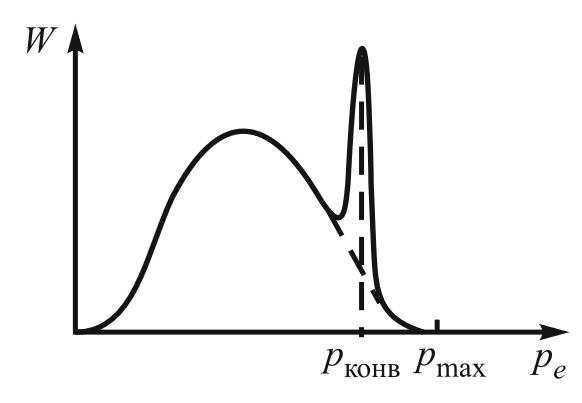
\includegraphics[width=\linewidth]{beta_shape.png}
  \caption{
    Форма спектра $\beta$-частиц при разрешённых переходах.
  }
  \label{img::beta_shape}
\end{wrapfigure}

где $B = \frac{16\pi^2}{c^4}D$. В нерелятивистском приближении, которое и имеет
место в нашем случае, выражение \eqref{eq::dNdEex} упрощается, и мы имеем

\begin{equation}\label{eq::dNdE}
\frac{dN}{dE} \approx \sqrt{E}(E_e - E)^2.
\end{equation}

Выражение \eqref{eq::dNdE} приводит к спектру, имеющему вид широкого колокола (рис
\ref{img::beta_shape}). Кривая плавно отходит от нуля и столь же плавно, по параболе,
касается оси абсцисс в области максимальной энергии электронов $E_e$.

Дочерние ядра, возникающие в результате $\beta$-распада, нередко оказываются
возбуждёнными. Возбуждённые ядра отдают свою энергию либо излучая $\gamma$-квант
(энергия которого равна разности энергий начального и конечного уровней), либо
передавая избыток энергии одному из электронов с внутренних оболочек атома.
Излучаемые в таком процессе электроны имеют строго определённую энергию и
называются конверсионными.

Конверсия чаще всего происходит на оболочках $K$ или $L$. На спектре,
представленном на рис. \ref{img::beta_shape}, видна монохроматическая линия,
вызванная электронами конверсии. Ширина этой линии в нашем случае является чисто
аппаратурной, по ней можно оценить разрешающую силу спектрометра.

